\textbf{Цель работы:} \\\indent
1) измерение частоты колебаний и длины волны при резонансе 
зуковых колебаний в газе, заполняющем трубу;\\\indent
2) определение показателя адиабаты с помощью уравнения состояния
идеального газа.\\ \indent
\textbf{Оборудование:} звуковой генератор, электронный осциллограф, 
микрофон, телефон, раздвижная труба, теплоизолированная турба, 
баллон со сжатым углекислым газом, газгольдер.\\ 

\section*{Теоретические сведения}

Скорость звука в газах поределяется как:
\begin{equation}
    c = \sqrt{\gamma \frac{R T}{\mu}}
\end{equation}

Если длина трубы $L$ равна целому числу полуволн ($L = n\frac{\lambda}{2}$),
волна, отраженная от торца трубы совпадает по фазе с падающей. Поэтому 
они усиливают друг друга и возникает резонанс. Скорость звука при 
этом связана с длиной волны как: 
\begin{equation}
   c = \lambda f
\end{equation}
\indent
Рассмотрим 2 способа образования резонансая:\\\indent
1)При $f = const$, изменяя длину трубы.\\\indent
2)При $L = const$, изменяя частоту звуковых колебаний. Тогда
\begin{align}
    L &= \frac{\lambda_1}{2} n = \frac{\lambda_2}{2} (n+1)\dots = \frac{\lambda_{\text{k+1}}}{2}(n + k)\\
    f_1 &= \frac{c}{\lambda_1} = \frac{c}{2L} n\\
    f_2 = \frac{c}{2L}(n + 1) &= f_1 + \frac{c}{2L} k \Rightarrow f_{\text{k+1}} = f_1 + \frac{c}{2L} k
\end{align}

\section*{Экспериментальная установка}
Звуковые колебания возбуждаются телефоном Т и улавливаются микрофоном М. 
Возникающий в нем сигнал отображается на осциллографе ЭО. 

\begin{figure}
    \centering
    \begin{subfigure}{0.45\linewidth}
        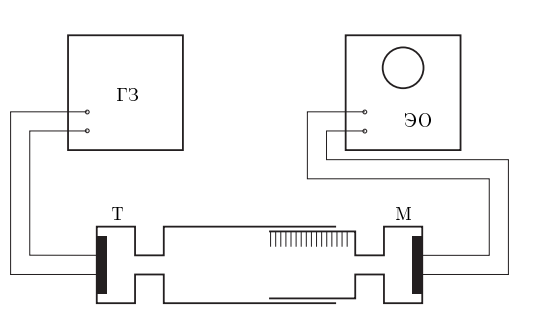
\includegraphics[width=9cm]{setup1.png}
        \caption{Установка для измерения скорости звука при подвижной трубе}
    \end{subfigure}
\hfill
    \begin{subfigure}{0.45\linewidth}
        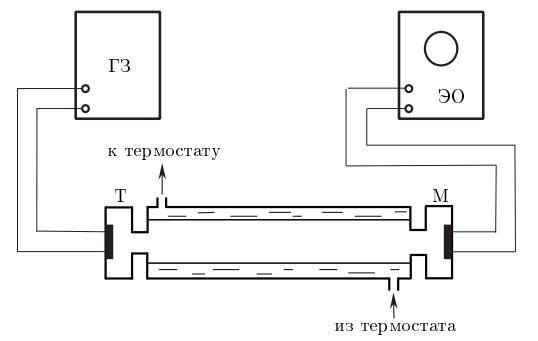
\includegraphics[width=9cm]{setup2.png}
        \caption{Установка для изучения зависимости скорости звука от температуры}
    \end{subfigure}
\end{figure}



\newpage

\section*{Экспериментальные данные}
\subsection*{Для воздуха:}
\begin{table}[h!]
    \centering
    \begin{tabular}{|c|c|c|c|c|c|c|c|c|}
        \hline
        № &1 & 2 & 3 & 4 & 5 & 6 & $\lambda$ см & $c$ м/с \\\hline
        $L$, см ($\nu = 3750$ Гц) & 3 & 7.6 & 12.3 & 16.7 & - & -  &9.2 & 344  \\\hline
        $L$, см ($\nu = 5500$ Гц) & 1.2& 4.3 &7.5 & 10.5 & 13.7 & 16.8 & 6.2 & 343  \\\hline
        $L$, см ($\nu = 4750$ Гц) & 1.9& 5.5 & 9.2 & 12.8 &16.3 & - & 7.7 &  345 \\\hline
        $L$, см ($\nu = 4500$ Гц) & 2& 5.8 &9.6 & 12.7 & 16.3 & -& 7.2 & 341  \\\hline
    \end{tabular}
    \caption{Зависимость длины трубы от номера резонанса в воздухе}
\end{table}

\begin{figure}[h!]
    \centering
    \begin{subfigure}{0.45\textwidth}
        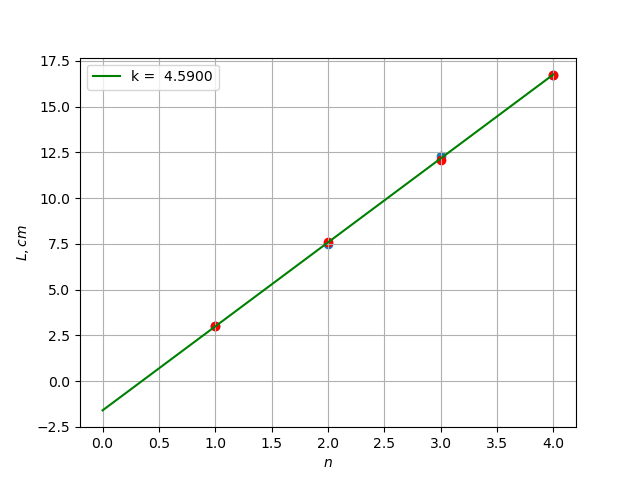
\includegraphics[height=5cm]{plot1.png}
        \subcaption{Зависимость длины от номера резонанса при $\nu = 3750$ Гц}
    \end{subfigure}
\hfill
    \begin{subfigure}{0.45\textwidth}
        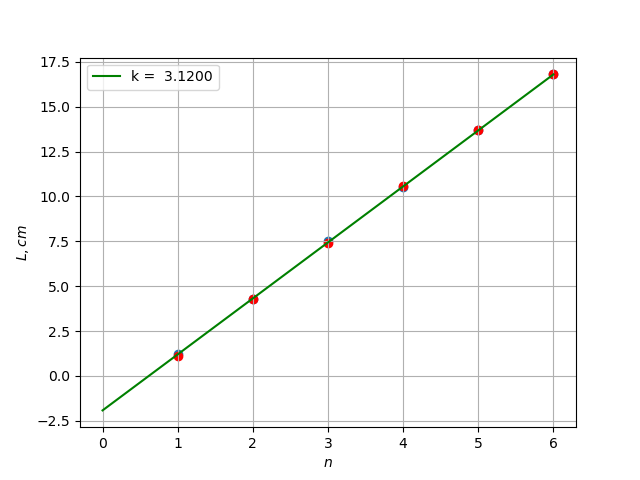
\includegraphics[height=5cm]{plot2.png}
        \subcaption{Зависимость длины от номера резонанса при $\nu = 5500$ Гц}
    \end{subfigure}
    \begin{subfigure}{0.45\textwidth}
        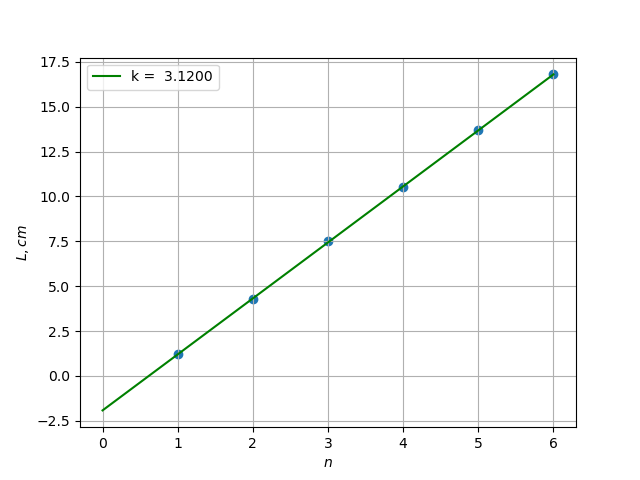
\includegraphics[height=5cm]{plot3.png}
        \subcaption{Зависимость длины от номера резонанса при $\nu = 4500$ Гц}
    \end{subfigure}
    \begin{subfigure}{0.45\textwidth}
        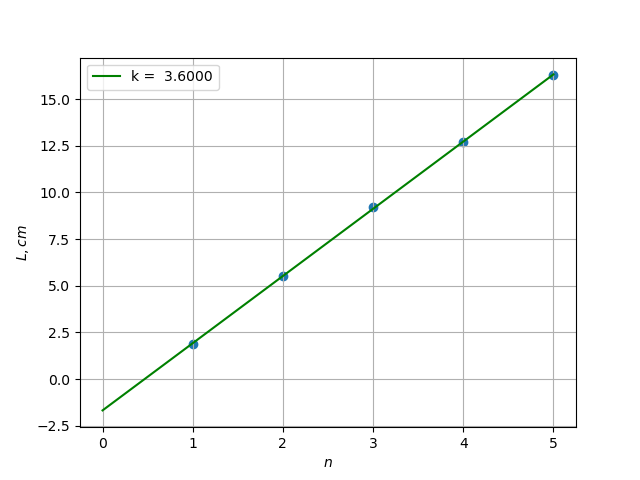
\includegraphics[height=5cm]{plot4.png}
        \subcaption{Зависимость длины от номера резонанса при $\nu = 4750$ Гц}
    \end{subfigure}

\end{figure}

\newpage

\subsection*{Для CO_2:}
\begin{table}[h!]
    \centering
    \begin{tabular}{|c|c|c|c|c|c|c|c|c|}
        \hline
        № &1 & 2 & 3 & 4 & 5 & $\lambda$ см & $c$ м/с \\\hline
        $L$, см ($\nu = 1500$ Гц) & 16.2 & 6 & - & - & -  &20.4 & 306  \\\hline
        $L$, см ($\nu = 2000$ Гц) & 21.2& 15.6 &8.7 & 1.7 & -  & 13 & 261 \\\hline
        $L$, см ($\nu = 2500$ Гц) & 20.7& 13.8 & 10.2 & 4.5 &- & 10.4 & 261 \\\hline
        $L$, см ($\nu = 3000$ Гц) & 20.1& 15.7 &10.7 & 6.3 & 1.1 & 9.48& 284  \\\hline
    \end{tabular}
    \caption{Зависимость длины трубы от номера резонанса в углекислом газе}
\end{table}

\begin{figure}[h!]
    \centering
    \begin{subfigure}{0.45\textwidth}
        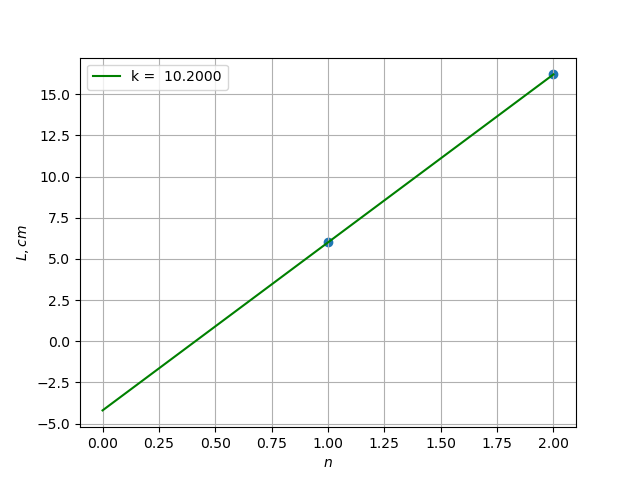
\includegraphics[height=5cm]{plotc1.png}
        \subcaption{Зависимость длины от номера резонанса при $\nu = 1500$ Гц}
    \end{subfigure}
\hfill
    \begin{subfigure}{0.45\textwidth}
        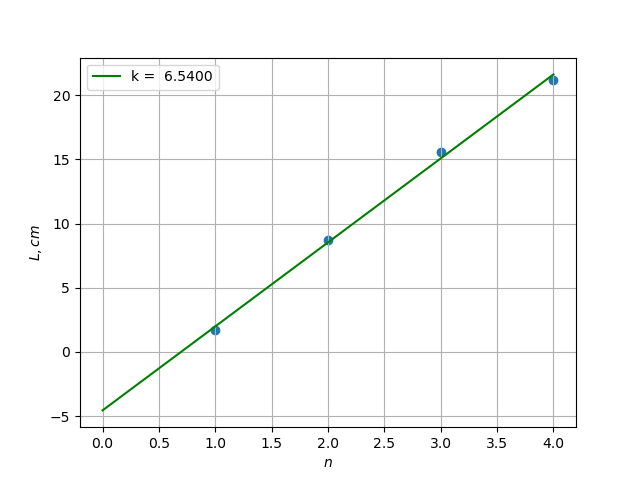
\includegraphics[height=5cm]{plotc2.png}
        \subcaption{Зависимость длины от номера резонанса при $\nu = 2000$ Гц}
    \end{subfigure}
    \begin{subfigure}{0.45\textwidth}
        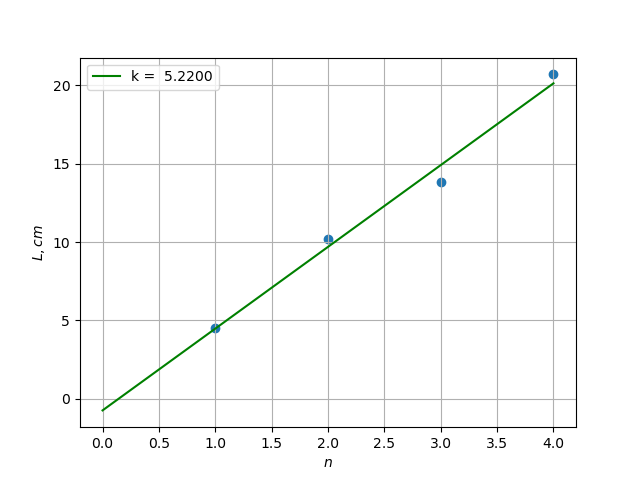
\includegraphics[height=5cm]{plotc3.png}
        \subcaption{Зависимость длины от номера резонанса при $\nu = 4500$ Гц}
    \end{subfigure}
    \begin{subfigure}{0.45\textwidth}
        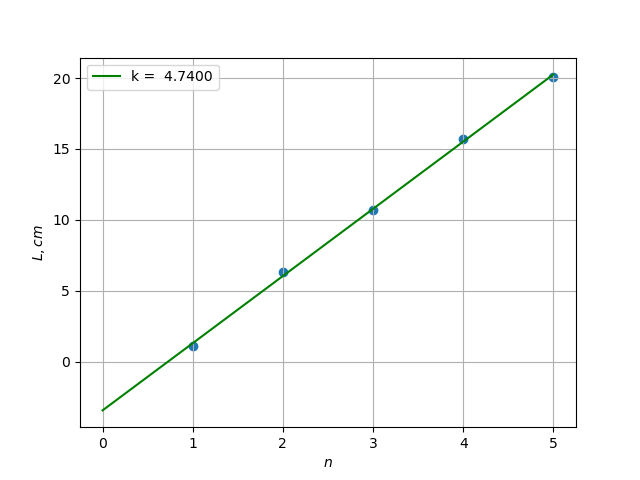
\includegraphics[height=5cm]{plotc4.png}
        \subcaption{Зависимость длины от номера резонанса при $\nu = 4750$ Гц}
    \end{subfigure}

\end{figure}

Теперь найдем коэффициент $\gamma = C_p / C_v$:
\begin{table}
    \centering
    \begin{tabular}{|c|c|c|c|c|c|c|c|}
        \hline
        1 & 2 & 3 & 4 & 5 & $T^{\circ}C$ & $c$ м/c & \gamma \\\hline
        275 & 495 & 735 & 995 & 1225 & 18 & 335 & 2.14\\\hline
        765& 1015& 1265& 1515 & 1775 & 40 & 362 & 2.32\\\hline
        524& 778& 1038& 1298& 1558 & 55 & 362 & 2.21\\\hline
    \end{tabular}
    \caption{Частота при резонансе при разных температурах}
\end{table}

\begin{figure}[h!]
    \centering
    \begin{subfigure}{0.45\textwidth}
        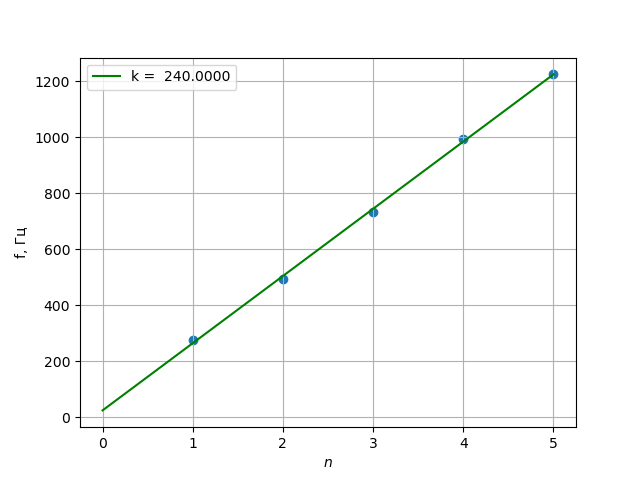
\includegraphics[height=5cm]{plotT1.png}
        \subcaption{Зависимость частоты от номера резонанса при $T = 18^{\circ}C$}
    \end{subfigure}
\hfill
    \begin{subfigure}{0.45\textwidth}
        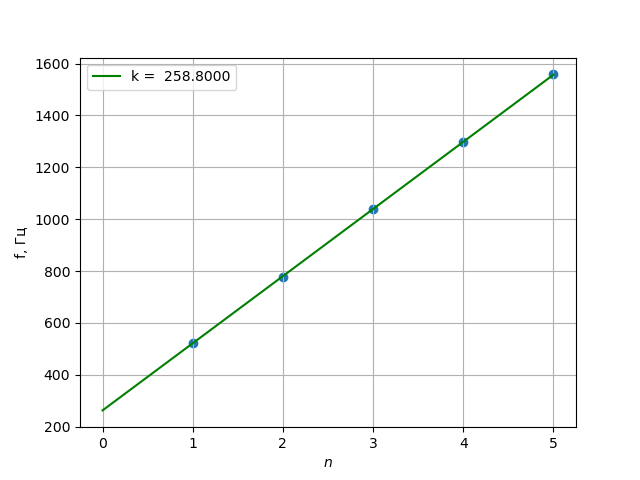
\includegraphics[height=5cm]{plotT2.png}
        \subcaption{Зависимость частоты от номера резонанса при $T = 40^{\circ}C$}
    \end{subfigure}
    \begin{subfigure}{0.45\textwidth}
        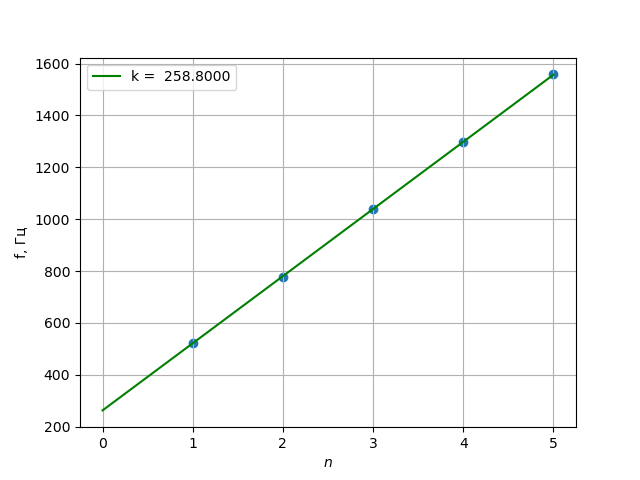
\includegraphics[height=5cm]{plotT3.png}
        \subcaption{Зависимость частоты от номера резонанса при $T = 55^{\circ}C$}
    \end{subfigure}
\end{figure}


